\section{Adiabatic Factorization Algorithm}
\label{Section:AFA}

It is worth to start this section by stating something quite relevant about adiabatic factorization and Shor's algorithm. While the adiabatic approach allows us to implement the factorization, which is also the main goal of Shor's algorithm, it does not mean we are implementing the Shor's algorithm adiabatically. For this reason, we refer to this method as \textit{adiabatic factorization}.

The problem of integer factorization can be formulated as a constrained search over pairs of natural numbers $p$ and $q$ such that
\begin{equation}
	N = p \times q.
	\label{eq:integer_factorization}
\end{equation}
In the context of adiabatic quantum computation we aim to encode this constraint into the ground state of a problem Hamiltonian, allowing the solution to emerge through adiabatic evolution.

To encode candidate solutions $p$ and $q$, we adopt a binary representation of natural numbers. Any natural number $N$ can be expressed as:
\begin{equation}
	N = \sum_{j=0}^{n_\text{bits} - 1} 2^j x_j,
	\label{eq:binary_integer}
\end{equation}
where each $x_j \in \{0,1\}$ and the bit string $\mathbf{x} = x_{n_\text{bits}-1} \dots x_0$ represents the binary encoding of $N$. In their approach, Peng et al.~\cite{peng_quantum_2008} exploit the fact that the factors $p$ and $q$ of an odd composite number can be rewritten as:
\begin{equation}
	\begin{cases}
		p = 2p' + 1 \\
		q = 2q' + 1
	\end{cases} .
	\label{eq:factors_simplification}
\end{equation}
It can be proved that the $n_p$ and $n_q$ are an upper bound on the number of qubits required to represent $p'$ and $q'$, respectively:
\begin{equation}
	\begin{cases}
		n_p = m\,\big(\lfloor \sqrt{N} \rfloor_o\big) - 1 \\[2ex]
		n_q = m\bigg(\left\lfloor \dfrac{N}{3} \right\rfloor \bigg) - 1
	\end{cases} ,
	\label{eq:factors_num_bits}
\end{equation}
where $\lfloor a \rfloor \big(\lfloor a \rfloor_o\big)$ denotes the largest (odd) integer not larger than a, while $m(b)$ denotes the smallest number of bits required for representing $b$~\cite{peng_quantum_2008}. Then, the adiabatic factorization algorithm will make use of $n = n_p + n_q$ qubits. The full quantum state 
\begin{equation}
	\ket{\Psi} = \ket*{\Psi_{p'}} \otimes \ket*{\Psi_{q'}},
	\label{eq:full_quantum_state}
\end{equation}
where $\ket*{\Psi_{p'}} = \ket*{\psi_{1}}\otimes \cdots \otimes \ket*{\psi_{n_p}}$ and $\ket*{\Psi_{q'}} = \ket*{\psi_{n_p+1}}\otimes \cdots \otimes \ket*{\psi_{n_p +n_q}}$.

To encode the factorization constraint into the adiabatic quantum framework, we define the objective function as ~\cite{peng_quantum_2008}:
\begin{equation}
	f(p,q) = \big(N - p \times q \big)^2,
\end{equation}
such that its global minimum $f(p,q)=0$ corresponds to valid factors. Translating this into a Hamiltonian acting on the computational basis, we obtain the quadratic problem Hamiltonian:
\begin{equation}
	\hat{H}_\mathrm{QP} = \bigg[ N \1 - \bigg( \sum_{\ell=1}^{n_p} 2^\ell \hat{x}_\ell + \1 \bigg)
	\bigg( \sum_{m=1}^{n_q} 2^m \hat{y}_m + \1 \bigg) \bigg]^2\,,
	\label{eq:quadratic_problem_hamiltonian}
\end{equation}
where $\hat{x}_\ell = \dfrac{\1 - \hat{\sigma}_\ell^z}{2}$ and $\hat{y}_m = \dfrac{\1 - \hat{\sigma}_m^z}{2}$ are the number operators acting on the qubits encoding $p'$ and $q'$, respectively. The solution to the factorization problem is encoded in the ground state of $\hat{H}_\mathrm{QP}$.

The initial state of the system is prepared as:
\begin{equation}
	\ket{\psi(0)} = \ket{+}^{\otimes n}\,,
	\label{eq:initial_state}
\end{equation}
where $\ket{+} = \frac{1}{\sqrt{2}} (\ket{0} + \ket{1})$ is the eigenstate of $\hat{\sigma}^x$, corresponding to the ground state of the initial Hamiltonian $\hat{H}_0$ defined in Eq.~\ref{eq:transverse_field_hamiltonian}.
Following the adiabatic theorem, if the evolution from $\hat{H}_0$ to $\hat{H}_\mathrm{QP}$ is slow enough, the system will remain in the instantaneous ground state, reaching the ground state of $\hat{H}_\mathrm{QP}$ at the end of the protocol. This final state encodes the solution to the factorization problem.

Despite its conceptual clarity, the Hamiltonian $\hat{H}_\mathrm{QP}$ includes high-order multiqubit interactions, such as three- and four-body terms of the form $\hat{\sigma}_\ell^z \hat{\sigma}_m^z \hat{\sigma}_k^z$ and $\hat{\sigma}_\ell^z \hat{\sigma}_m^z \hat{\sigma}_k^z \hat{\sigma}_n^z$. These many-body interactions are difficult to implement, since they require one to bring all involved qubits together and make them interact in a controlled way, resulting in prone-to-error processes. The need to avoid those terms is of pivotal interest to provide efficient quantum algorithms.

\section{Digitized Adiabatic Quantum Factorization}
Although the adiabatic model is often formulated in terms of continuous time evolution, it can be simulated efficiently using gate-based quantum computation through a process known as digitization.

In the digitized approach, the continuous adiabatic evolution governed by a time-dependent Hamiltonian as of Eq.~\ref{eq:adiabatic_passage} is approximated by a sequence of quantum gates through trotterization, breaking the total evolution into small time slices. Each slice is implemented as a layer in a quantum circuit, simulating the adiabatic trajectory step by step.

This method was successfully demonstrated by Hegade et al.~\cite{hegade_digitized_2021}, where the authors implemented a digitized adiabatic factorization algorithm on superconducting hardware. They successfully factorized numbers $N=21$, $N=91$, and $N=217$, and also proved enhancements by introducing an additional layer in the algorithm due to application of counter-diabatic driving theories.

\subsubsection{QAOA for Standard Adiabatic Factorization}
In some sense, we can say that QAOA can be viewed as a shortcut to adiabaticity implemented in the circuit model for quantum computation. Rather than performing a slow, continuous evolution, QAOA uses a fixed-depth quantum circuit composed of alternating unitaries derived from the mixing and problem Hamiltonians. The parameters of these unitaries are optimized variationally to prepare a state that approximates the solution.

Díez-Valle et al.~\cite{diez-valle_universal_2025} demonstrate that QAOA and quantum annealing share fundamental structural features. Their results provide strong evidence that smooth annealing paths can be reconstructed from the optimal parameters of QAOA, reinforcing the view of QAOA as a digitized, variationally optimized form of adiabatic evolution.

In summary, the ingredients to build and execute the QAOA algorithm applied to integer factorization --- or what we will call the ``\texttt{standard} protocol'' --- are:
\begin{itemize}
    \item A Hamiltonian $\hat{H}_\mathrm{QP}$ (Eq.~\ref{eq:quadratic_problem_hamiltonian}) that encodes the solution to the factorization problem in its ground state.
    \item A mixing Hamiltonian $\hat{H}_\mathrm{M}$ that does not commute with $\hat{H}_\mathrm{QP}$, e.g., Eq.~\ref{eq:mixing_hamiltonian}.
    \item A quantum circuit that implements the state evolution given by Eq.~\ref{eq:qaoa_state_evolution}.
    \item A classical optimizer to find the circuit's optimal parameters.
    \item A cost function given by $F_p (\bm{\gamma}, \bm{\beta}) = \bra{\psi_p (\bm{\gamma}, \bm{\beta})} \hat{H}_\mathrm{QP} \ket{\psi_p (\bm{\gamma}, \bm{\beta})}$.
\end{itemize}

Due to the form of Eq.~\ref{eq:quadratic_problem_hamiltonian}, the problem Hamiltonian can be expressed as:
\begin{equation}
    \hat{H}_\mathrm{QP} = n \1 + \sum_i a_i \hat{\sigma}^z_i
    + \sum_{ij} b_{ij} \hat{\sigma}^z_i \hat{\sigma}^z_j
    + \sum_{ijk} c_{ijk} \hat{\sigma}^z_i \hat{\sigma}^z_j \hat{\sigma}^z_k
    + \sum_{ijk\ell} d_{ijk\ell} \hat{\sigma}^z_i \hat{\sigma}^z_j \hat{\sigma}^z_k \hat{\sigma}^z_\ell
    \label{eq:expanded_problem_quadratic_hamiltonian}
\end{equation}
Then, the part of $e^{-i \gamma \hat{H}_\mathrm{QP}}$ corresponding to the term $a_i \hat{\sigma}^z_i$ is
\begin{equation}
    e^{-i \gamma a_i \hat{\sigma}^z_i} = e^{-i \gamma a_i} \ket{0}\bra{0}
    + e^{i \gamma a_i} \ket{1}\bra{1}
    = R_Z(2 \gamma a_i)\,,
\end{equation}
the part corresponding to $b_{ij} \hat{\sigma}^z_i \hat{\sigma}^z_j$ is
\begin{equation}
    \begin{split}
        e^{-i \gamma b_{ij} \hat{\sigma}^z_i \hat{\sigma}^z_j} \\
         &=e^{-i\gamma b_{ij}} \ket{00}\bra{00} + e^{i\gamma b_{ij}} \ket{10}\bra{10}
        +  e^{i\gamma b_{ij}} \ket{01}\bra{01} + e^{-i\gamma b_{ij}} \ket{11}\bra{11} \\
        &= R_{ZZ} (2 \gamma b_{ij})\,,
    \end{split}
\end{equation}
and so on for the higher-order terms. Similarly, the mixing Hamiltonian $\hat{H}_\mathrm{M}$ gives rise to individual X-rotations at the end of each QAOA layer. With all this, one constructs the QAOA circuit --- such as the circuit shown in Fig.~\ref{fig:standard_circuit} used for factorization of the number $N=35$.

\begin{figure}[h]
    \centering
    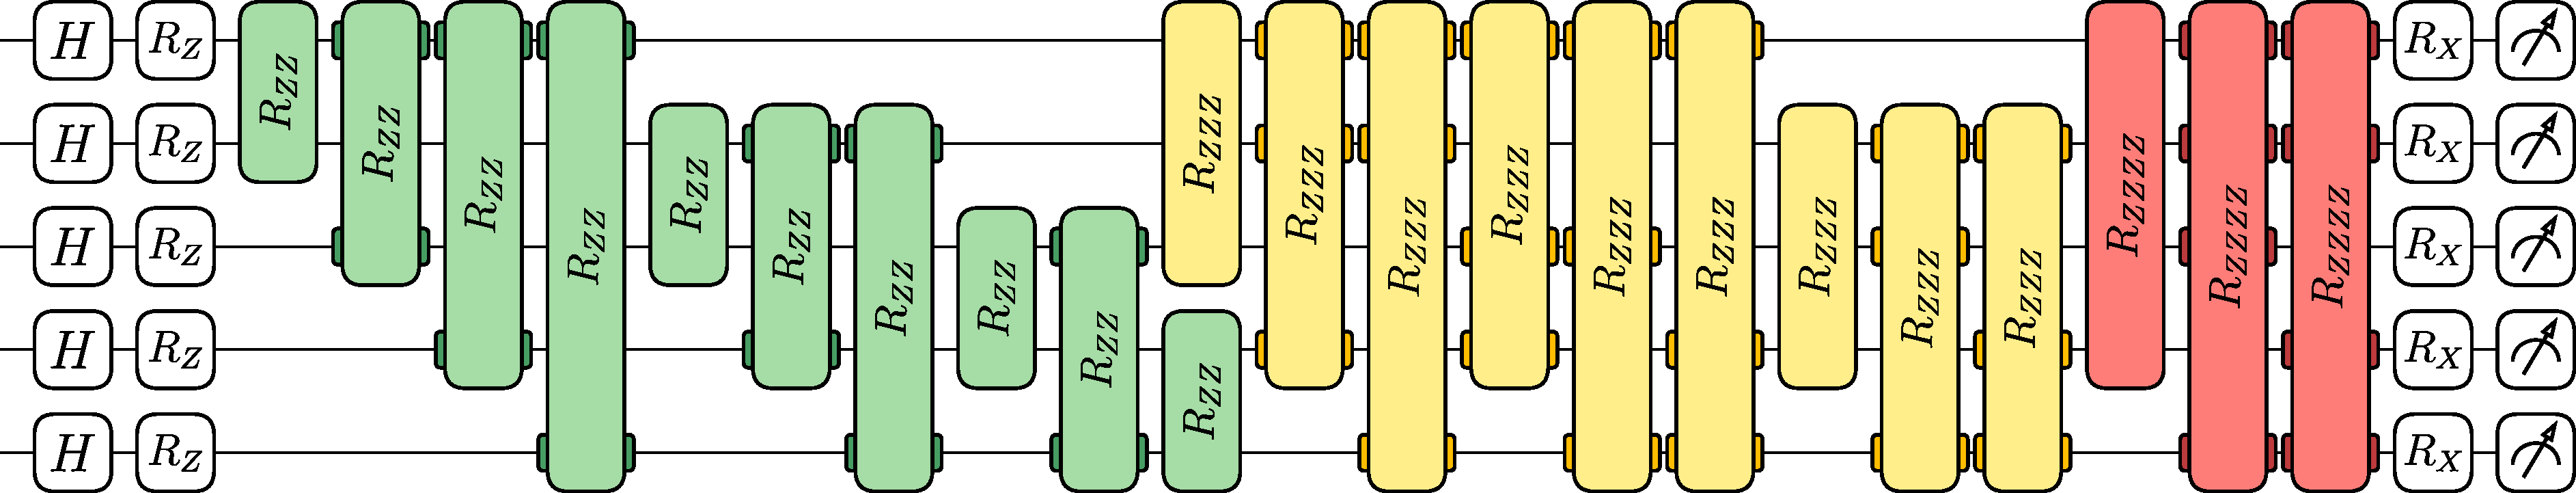
\includegraphics[width=1\textwidth]{02-factorization/figs/standard_circuit_35.pdf}
    \caption{One-layer circuit for factorizing the number $N=35$ using the standard QAOA protocol. Notice the presence
    of three- and four-qubit gates, highlighted in yellow and red, respectively. Rotation angles are omitted for simplicity.}
    \label{fig:standard_circuit}
\end{figure}

A related study by Anschuetz et al.~\cite{anschuetz_variational_2018} applies a similar method, combined with additional preprocessing and simplifications, to factor numbers as large as $291311$. Building on this idea, Karamlou et al.~\cite{karamlou_analyzing_2021} used classical preprocessing heuristics to factor $1099551473989$, $3127$, and $6557$ using only $3$, $4$, and $5$ qubits, respectively. In contrast, our goal is not to optimize for specific instances, but rather to analyze the general, standard approach to quantum factorization without relying on ad-hoc techniques. The motivatioin comes from establishing a broadly applicable framework, valid for any input $N$, while avoiding the need for modifications to the underlying factorization algorithm.

\subsection{QAOA for Linearized Adiabatic Factorization}
As mentioned in the introduction to Section~\ref{Section:AFA}, the adiabatic factorization algorithm
needs to deal with the difficulty of implementing three- and four-body interaction terms. In the 
digitized version of this problem, like QAOA, this difficulty is bypassed by assuming that all three- and four- qubit gates --- see e.g. Fig.~\ref{fig:standard_circuit} --- can be efficiently implemented in a digital computer. However, for universal computers available so far, these gates are not efficiently implemented and we need to decompose them in multiple two-qubit gates, as shown in Fig.~\ref{fig:gate_decomposition}, what might result in lower fidelities at the end of the quantum circuit in a real scenario.

\begin{figure}[h]
    \centering
    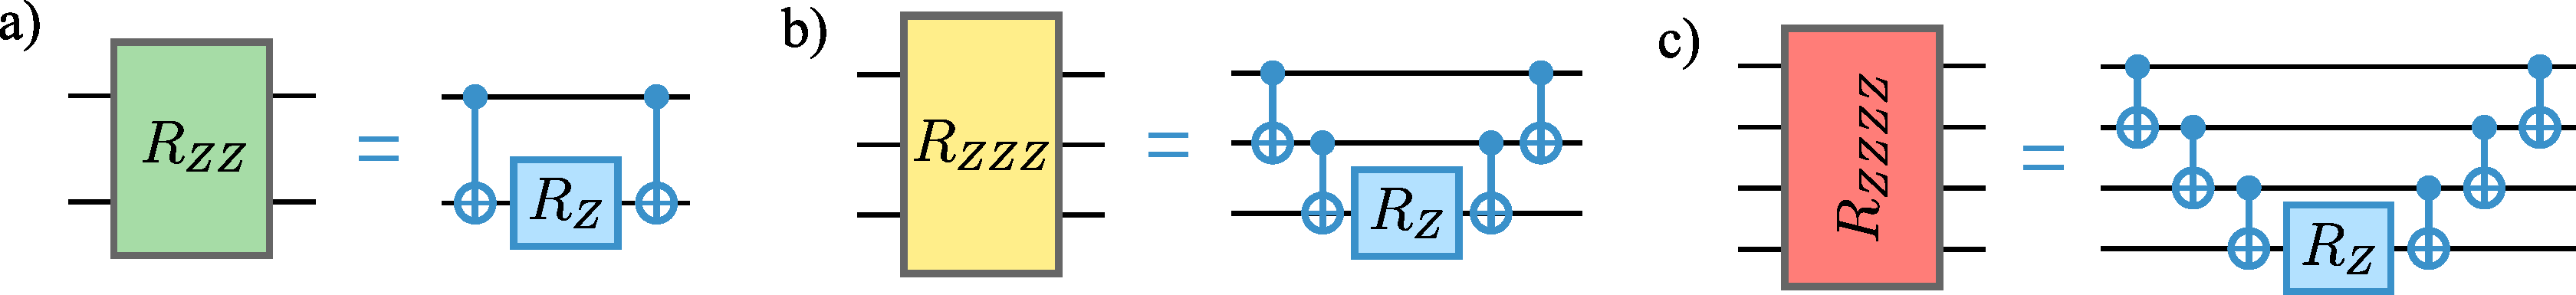
\includegraphics[width=1\textwidth]{02-factorization/figs/gate_decomposition.pdf}
    \caption{Decomposition of (a) two-, (b) three-, and (c) four-qubit Z-rotation gates in CNOTs and
    single-qubit Z-rotations.}
    \label{fig:gate_decomposition}
\end{figure}

To mitigate this issue, we propose a linearized problem Hamiltonian inspired by the same factorization condition, defined as:
\begin{equation}
	\hat{H}_\mathrm{LP} = N \1 - \bigg( \sum_{\ell=1}^{n_p} 2^\ell \hat{x}_\ell + \1 \bigg)
	\bigg( \sum_{m=1}^{n_q} 2^m \hat{y}_m + \1 \bigg)\,.
	\label{eq:linear_problem_hamiltonian}
\end{equation}
Unlike the original Hamiltonian $\hat{H}_\mathrm{QP}$, whose ground state encodes the solution, $\hat{H}_\mathrm{LP}$ contains only two-body terms and is therefore easier to implement, but the factorization solution corresponds to an eigenstate with eigenvalue zero rather than the ground state. Since the adiabatic theorem is not restricted to ground states but applies to any non-degenerate eigenstate, we hypothesize that it is possible to target this eigenstate through a suitable adiabatic or variational process. Based on this idea, our proposal is to replace the original Hamiltonian in the QAOA layers with $\hat{H}_\mathrm{LP}$, leveraging the possibility of starting from an eigenstate near the middle of the initial Hamiltonian’s spectrum and evolving under $\hat{H}_\mathrm{LP}$ to preserve this eigenstate structure, ultimately reaching the correct factorization solution, which also lies near the center of the spectrum.

\begin{figure}[h]
    \centering
    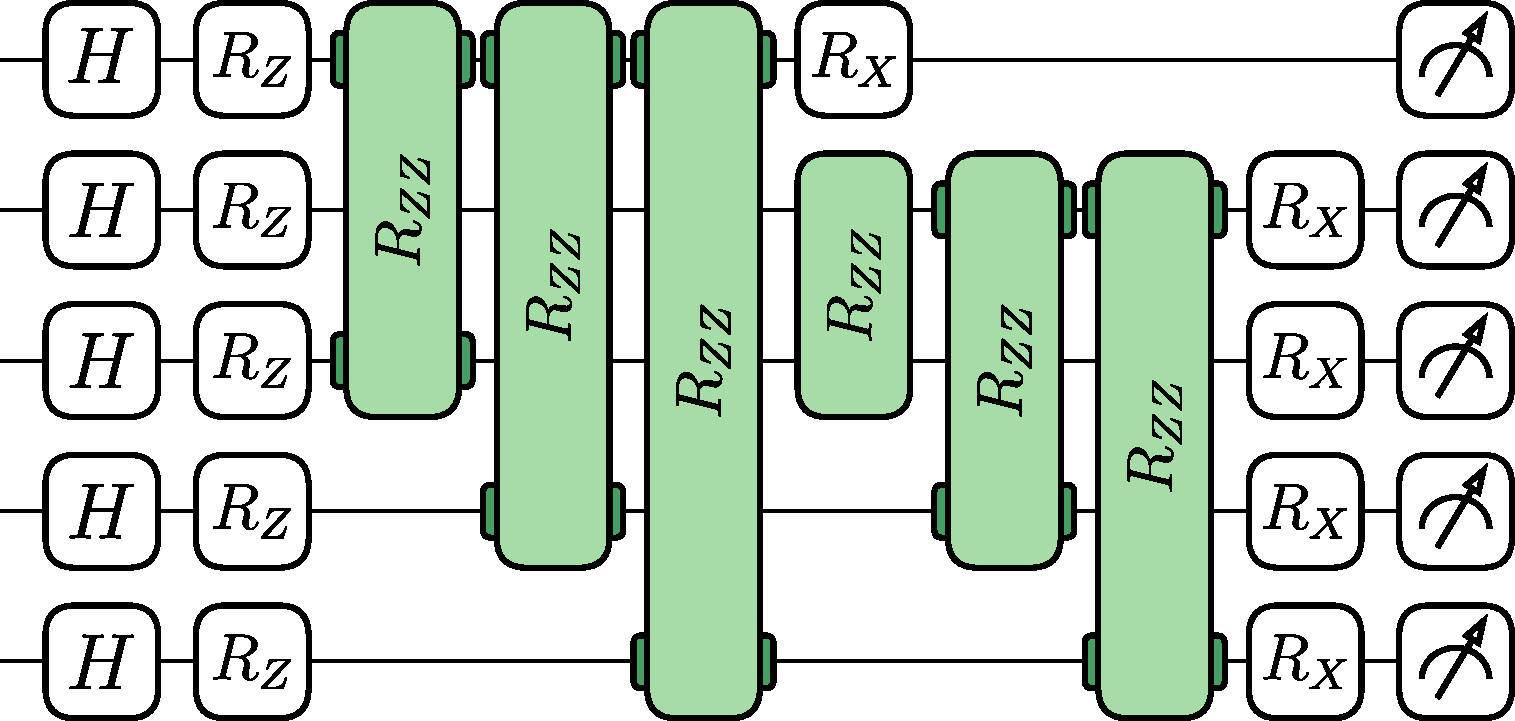
\includegraphics[width=0.45\textwidth]{02-factorization/figs/linear_circuit_35.pdf}
    \caption{One-layer circuit for factorizing the number $N=35$ using our protocol, evolving the state with the linear Hamiltonian $H_{\mathrm{LP}}$. Notice the simplification with respect to Fig.~\ref{fig:standard_circuit}
    due to the absence of three- and four-qubit gates.}
    \label{fig:linear_circuit_35.pdf}
\end{figure}